\begin{multicols}{2}
    \begin{figure}[H]
        \centering
        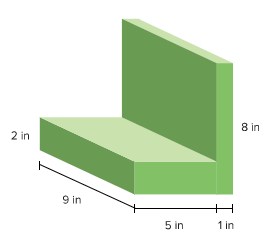
\includegraphics[width=0.5\linewidth]{../images/20230316201422}
        \caption{}
        \label{fig:20230316201422}
    \end{figure}
    \columnbreak
    \question[10] La Figura \ref{fig:20230316201422} está formada por 2 prismas rectangulares.
    \textbf{¿Cuál es el volumen de esta figura?}
\end{multicols}
% \end{minipage}\hfill
% \begin{minipage}{0.7\linewidth}
\begin{solutionbox}{16cm}
    \begin{minipage}[t]{.3\textwidth}
        \begin{figure}[H]
            \centering
            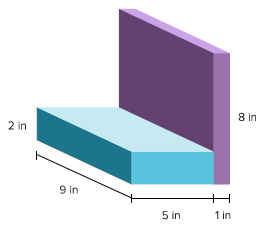
\includegraphics[width=0.9\linewidth]{../images/20230316201857}
            \caption{Descomposicion de la Figura \ref{fig:20230316201422} en dos.}
            \label{fig:20230316201857}
        \end{figure}
    \end{minipage}\hfill
    \begin{minipage}[t]{.55\textwidth}
        Podemos pensar en esta figura como 2 prismas rectangulares pegados (ver Figura \ref{fig:20230316201857}). Encontremos el volumen de cada prisma por separado.\\
        El volumen de un prisma rectangular es igual al largo $x$, por el ancho $y$, por la altura $z$:
        \[ V = xyz \]

        Para uno de los prismas, como el que aparece en la Figura \ref{fig:20230316202402}, se sabe que:\\
        \[ V = 5\times 9\times 2=90\]
        Volumen del prisma color turquesa es 90 pulgadas cúbicas.\\

        Para la segunda sección del prisma, como en la Figura \ref{fig:20230316205119}, se sabe que:\\
        \[ V = 1\times 9\times 8=72\]
        Volumen del prisma color púrpura es 72 pulgadas cúbicas.\\
        Ahora sumamos para obtener el volumen de toda la figura.
        \[ V_T = 90+72= 162\]
        Volumen de toda la figura $V_T$ es $162$ pulgadas cúbicas
    \end{minipage}
    \begin{multicols}{2}
        \begin{figure}[H]
            \centering
            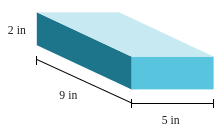
\includegraphics[width=0.6\linewidth]{../images/20230316202402}
            \caption{Primera sección del prisma de la Figura \ref{fig:20230316201422}}
            \label{fig:20230316202402}
        \end{figure}
        \columnbreak
        \begin{figure}[H]
            \centering
            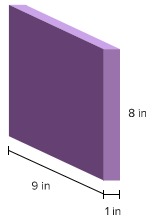
\includegraphics[width=0.3\linewidth]{../images/20230316205119}
            \caption{Segunda sección del prisma de la Figura \ref{fig:20230316201422}}
            \label{fig:20230316205119}
        \end{figure}
    \end{multicols}
\end{solutionbox}
% \end{minipage}


